\documentclass[12pt, letter]{exam}
\usepackage[utf8]{inputenc}
\usepackage[T1]{fontenc}
\usepackage[spanish]{babel}
\usepackage[autostyle,spanish=mexican]{csquotes}
\usepackage{amsmath}
\usepackage{amsthm}
\usepackage{physics}
\usepackage{tikz}
\usepackage{float}
\usepackage{siunitx}
\usepackage{multicol}
\usepackage{enumitem}
\usepackage[left=2.00cm, right=2.00cm, top=2.00cm, 
     bottom=2.00cm]{geometry}
\usepackage{pdfpages}

% \renewcommand{\questionlabel}{\thequestion}
\decimalpoint

\setlength{\belowdisplayskip}{-0.5pt}

\usepackage{tasks}
\settasks{
    label=\Alph*), 
    label-align=left,
    item-indent={20pt}, 
    column-sep={4pt},
    label-width={16pt},
}

\sisetup{per-mode=symbol}
\footer{}{\thepage}{}

\newcommand{\Fahrenheit}[1]{{#1}^{\circ} \,  \text{F}}

\begin{document}
\includepdf[pages={1}]{Caratula_Examen_Parcial_03_PU_Fisica_3_02_Grupo_43.pdf}

\newpage

\begin{questions}
    \section{(2 puntos) Dinámica.}

    \question \textbf{(1 punto)} \label{Problema_01} \textbf{Problema de ejecución: } Calcula la distancia a la que se deben de colocar dos masas, la primera de \SI{100}{\kilo\gram} y la segunda de \SI{1000}{\kilo\gram} para que se atraigan con una fuerza de \SI{1}{\newton}.
    \begin{tasks}(4)
        \task $\SI{1.167d-5}{\meter}$
        \task $\SI{6.67d-9}{\meter}$
        \task $\SI{6.67d-6}{\meter}$
        \task $\SI{2.582d-3}{\meter}$
    \end{tasks}
    \question \textbf{(1 punto)} La segunda ley de Newton relaciona la fuerza de manera directamente proporcional con dos cantidades:
    \begin{multicols}{2}
    \begin{tasks}
        \task Masa y peso.
        \task Masa y velocidad.
        \task Masa y aceleración.
        \task Aceleración y distancia.
    \end{tasks}
    \end{multicols}
    

    \section{(8 puntos) Electricidad.}

    \question \textbf{(1 punto)} Relaciona las unidades de las siguientes cantidades, una columna con la otra.
    \\
    \begin{minipage}[t]{0.4\linewidth}
        \begin{enumerate}[label=\arabic*)]
            \item Corriente.
            \item Resistencia.
            \item Voltaje.
        \end{enumerate}
    \end{minipage}
    \begin{minipage}[t]{0.4\linewidth}
        \begin{enumerate}[label=\alph*)]
            \item Ohm (\si{\ohm})
            \item Tesla (T)
            \item Ampere (\si{\ampere})
            \item Volt (\si{\volt})
        \end{enumerate}
    \end{minipage}
    \begin{tasks}(4)
        \task 1-c, 2-a, 3-d
        \task 1-d, 2-a, 3-c
        \task 1-a, 2-d, 3-c
        \task 1-a, 2-c, 3-b
    \end{tasks}
    \question \textbf{(1 punto)} \label{Problema_02} \textbf{Ejercicio de ejecución: } Determina la intensidad de la corriente eléctrica a través de una resistencia de \SI{1500}{\kilo\ohm} al aplicarle una diferencia de potencial de \SI{220}{\volt}.
    \begin{tasks}(4)
        \task \SI{1.466d-3}{\ampere}
        \task \SI{1.466d-4}{\ampere}
        \task \SI{1.466d-5}{\ampere}
        \task \SI{2.066d-5}{\ampere}
    \end{tasks}
    \question \textbf{(1 punto)} El flujo de las partículas cargadas en un conductor es lo que se conoce como \rule{2cm}{0.1mm}.
    \begin{tasks}(4)
        \task Voltaje.
        \task Corriente.
        \task Potencia.
        \task Resistencia.
    \end{tasks}
    \question \textbf{(1 punto)} Por experiencia sabemos que los materiales tienen un equilibrio en su carga eléctrica, es decir, son \rule{2cm}{0.1mm}.
    \begin{tasks}(4)
        \task Negativos.
        \task Positivos.
        \task Aislantes.
        \task Neutros.
    \end{tasks}
    \question \textbf{(1 punto)} Son aquellas plantas que generan electricidad por medio de la energía cinética de un volumen de agua:
    \begin{tasks}(4)
        \task Eólicas.
        \task Hidroeléctricas.
        \task Térmicas.
        \task Nucleares.
    \end{tasks}

    \newpage

    \question \textbf{(1 punto)} La capacidad de transmisión de energía eléctrica de una línea se determina por \rule{2cm}{0.1mm} de los conductores y \rule{2cm}{0.1mm} entre las torres.
    \begin{multicols}{2}
    \begin{tasks}
        \task la densidad - la forma.
        \task el diámetro - la altura.
        \task la capacidad de carga - la distancia.
        \task el material - la red.
    \end{tasks}
    \end{multicols}
    \question \textbf{(1 punto)} Nombre del científico a quien se le asocia el principio de inducción por el cual la energía mecánica de un generador se transforma en energía eléctrica.
    \begin{tasks}(4)
        \task Raleigh.
        \task Fermat.
        \task Faraday.
        \task Ampere.
    \end{tasks}
    \question \textbf{(1 punto)} La ley de inducción electromagnética establece que la variación \rule{2cm}{0.1mm} en una bobina induce \rule{2cm}{0.1mm}
    \begin{tasks}
        \task de la energía potencial - una corriente eléctrica.
        \task del flujo magnético - una corriente eléctrica.
        \task del flujo cinético - una corriente eléctrica.
        \task del flujo eléctrico - una intensidad magnética.
    \end{tasks}
    
    \section{(6 puntos) Calor, Trabajo y Energía.}
    
    \question \textbf{(1 punto)} En un problema de energía cinética se nos pide obtener la masa del objeto, ¿qué expresión es la que debemos de utilizar?
    \begin{tasks}(4)
        \task $m = \dfrac{v^{2}}{2 \, E_{k}}$
        \task $m = \dfrac{2}{E_{k} \, v^{2}}$
        \task $m = \dfrac{E_{k}}{2 \, v^{2}}$
        \task $m = \dfrac{2 \, E_{k}}{v^{2}}$
    \end{tasks}
    \question \textbf{(1 punto)} Es la capacidad de un sistema físico para realizar un trabajo:
    \begin{tasks}(4)
        \task Energía.
        \task Potencia.
        \task Movimiento.
        \task Fuerza.
    \end{tasks}
    \question \textbf{(1 punto)} La energía total de un sistema es:
    \begin{tasks}
        \task La suma de la energía potencial y la energía eléctrica.
        \task La suma de la energía potencial y la energía cinética.
        \task La diferencia de la energía potencial y la energía cinética.
        \task El producto de la energía potencial y la energía térmica.
    \end{tasks}
    \question \textbf{(1 punto)} El oro cambia de forma, es decir, pasa de su estado sólido a líquido a los $\Fahrenheit{1947.2}$. En grados Celsius ¿cuánto equivale esa temperatura?
    \begin{tasks}(4)
        \task \SI{2004}{\degreeCelsius}
        \task \SI{1804}{\degreeCelsius}
        \task \SI{1064}{\degreeCelsius}
        \task \SI{1004}{\degreeCelsius}
    \end{tasks}
    \question \textbf{(1 punto)} En la siguiente figura se presentan los mecanismos de transferencia de calor, identifica cada letra de la figura con el inciso correspondiente de cada mecanismo.
    \begin{figure}[H]
        \centering
        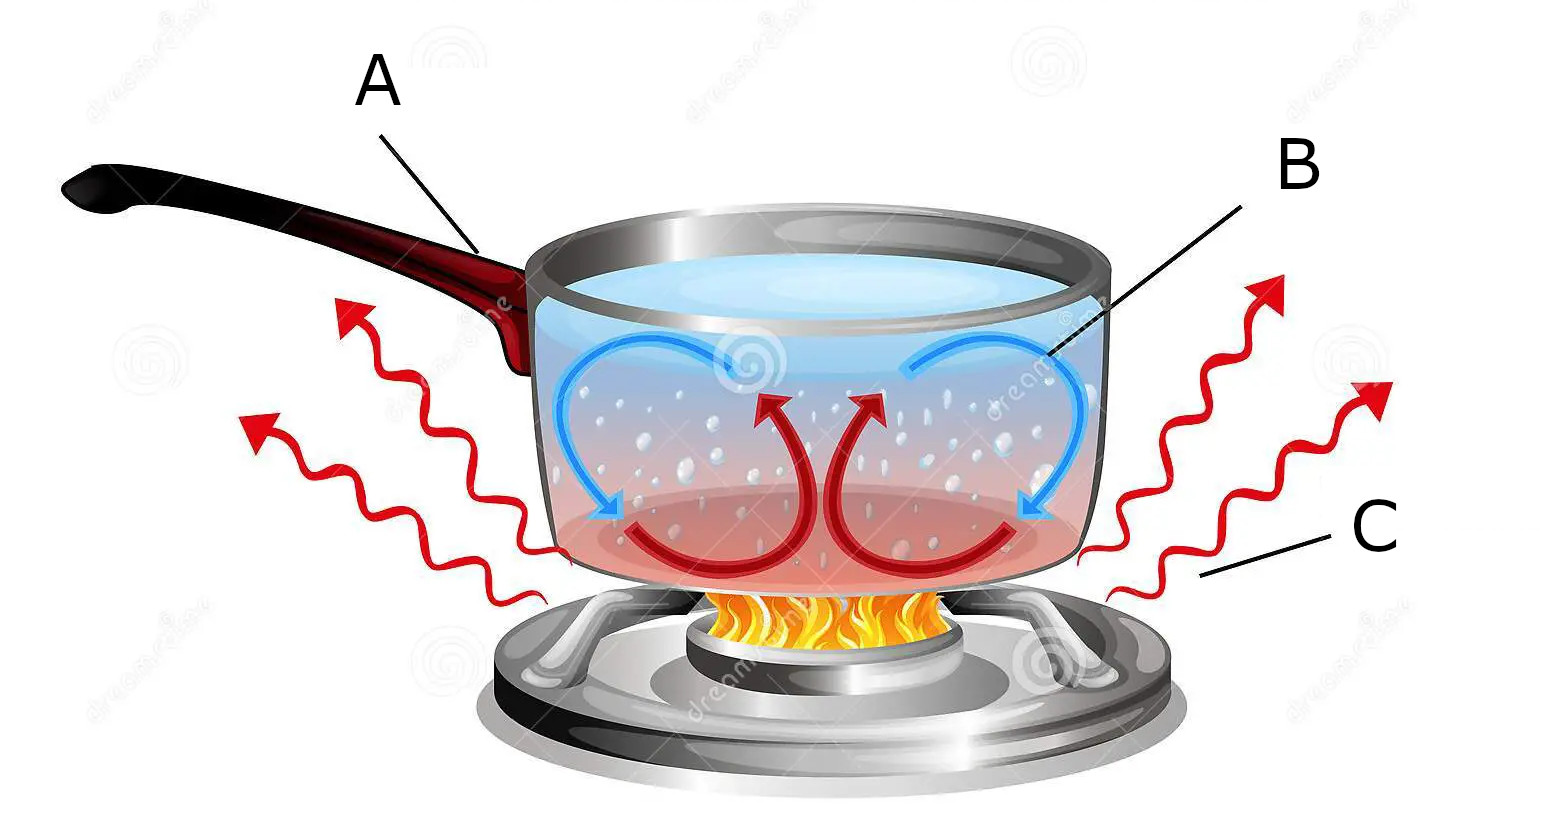
\includegraphics[scale=0.2]{Transferencia_Calor_01.jpg}
    \end{figure}
    \begin{multicols}{4}
    \begin{enumerate}[label=\Roman*)]
        \item Ebullición.
        \item Convección.
        \item Conducción.
        \item Radiación.
    \end{enumerate}
    \end{multicols}
    \begin{tasks}
        \task A - IV, B - I, C - II
        \task A - II, B - III, C - I
        \task A - I, B - II, C - III
        \task A - III, B - II, C - IV
    \end{tasks}
    \question \textbf{(1 punto)} \rule{2cm}{0.1mm} es una forma de energía que se transfiere entre dos sistemas (o entre partes de un sistema) debido a \rule{2cm}{0.1mm}.
    \begin{tasks}
        \task La energía cinética - al incremento de calor.
        \task El calor - una diferencia de temperatura.
        \task El calor - una suma de temperatura.
        \task La energía cinética - a un descenso de temperatura.
    \end{tasks}

    \section{(4 puntos) Transferencia de energía.}

    \question \textbf{(1 punto)} La eficiencia de una máquina ideal es:
    \begin{tasks}(4)
        \task $\eta < 100 \%$
        \task $\eta > 100 \%$
        \task $\eta = 100 \%$
        \task $\eta = 0 \%$
    \end{tasks}
    \question \textbf{(1 punto)} La eficiencia de una máquina (expresada en porcentaje) se define como:
    \begin{tasks}(4)
        \task $\eta = W_{e} \cdot W_{s}$
        \task $\eta = \dfrac{W_{e}}{W_{s}}$
        \task $\eta = \dfrac{W_{s}}{W_{e}}$
        \task $\eta = (W_{e})^2 (W_{s})^2$
    \end{tasks}

    \newpage

    \question \textbf{(1 punto)} Las máquinas reales experimentan pérdidas de energía, que en conformidad con la ley de conservación de energía, a menudo \rule{2cm}{0.1mm}
    \begin{multicols}{2}
    \begin{tasks}
        \task se transforma en electricidad.
        \task se disipan en forma de calor.
        \task aumentan su energía potencial.
        \task incrementan su velocidad angular.
    \end{tasks}
    \end{multicols}
    \question \textbf{(1 punto)} Un aerogenerador transforma la energía \rule{2cm}{0.1mm} del viento en energía eléctrica.
    \begin{tasks}(4)
        \task solar.
        \task calorífica.
        \task cinética.
        \task potencial.
    \end{tasks}
    % \question Una planta hidroeléctrica transforma la energía \rule{2cm}{0.1mm} del agua en energía eléctrica.
    % \begin{tasks}(4)
    %     \task potencial.
    %     \task cinética.
    %     \task nuclear.
    %     \task eólica.
    % \end{tasks}
\end{questions}

\vspace*{1cm}
\textbf{\huge{Formulario.}}
\begin{table}[H]
\centering
\setlength{\tabcolsep}{40pt}
\renewcommand{\arraystretch}{1.5}
\begin{tabular}{c  c}
    \multicolumn{2}{c}{Dinámica} \\
    $F = m \cdot a$ & $F = G \, \dfrac{m_{1} \cdot m_{2}}{r^{2}}$ \\
    $G = \displaystyle \SI[per-mode=fraction]{6.67d-11}{\newton\square\meter\per\square\kilo\gram}$ &  \\ \hline
    \multicolumn{2}{c}{Electricidad} \\
    $q = n \cdot e$ & $e = \SI{1.6d-19}{\coulomb}$ \\
    $V = I \cdot R$ & \\
    \hline
    \multicolumn{2}{c}{Calor, energía y trabajo} \\
    $T = F \cdot d$ & $g = \displaystyle \SI{9.81}{\meter\per\square\second}$ \\
    $E_{k} = \dfrac{1}{2} \, m \, v^{2}$ & $E_{p} = m \, g \, h$ \\
    $\unit{\degreeCelsius} = \dfrac{5}{9} \left( ^{\circ}\text{F} - 32 \right)$ & $^{\circ}\text{F} = \dfrac{9}{5} \, \unit{\degreeCelsius} + 32$ \\
    $K = \unit{\degreeCelsius} + 273.15$ & $\unit{\degreeCelsius} = K - 273.15$ \\
    $R = \, ^{\circ}\text{F} + 460$ & \\
\end{tabular}
\end{table}

\newpage

En este espacio deberás de incluir el desarrollo completo de los Problemas de Ejecución. El problema se califica de la siguiente manera: \textbf{a) Datos: 0.25 puntos}, \textbf{b) Expresión(es): 0.25 puntos}, \textbf{c) Sustitución: 0.25 puntos} y \textbf{d) Manejo de unidades: 0.25 puntos}.

\vspace*{0.5cm}
Solución al Problema de Ejecución \ref{Problema_01}:

\vspace*{5cm}
\rule{0.9\textwidth}{0.3mm}

Solución al Problema de Ejecución \ref{Problema_02}:

\end{document}